\documentclass[report,11pt]{elsarticle}
%\documentclass{article}[11pt,a4]
%\documentclass[11pt]{article}

\usepackage[lined,linesnumbered]{algorithm2e}
\usepackage{a4wide}
\usepackage{ae}
\usepackage[czech]{babel}
\usepackage{graphicx}
\usepackage{url}
\usepackage{pdfpages}

\paperwidth=210 true mm
\paperheight=297 true mm
\pdfpagewidth=210 true mm
\pdfpageheight=297 true mm

\usepackage[czech]{babel}
\selectlanguage{czech}


\begin{document}

\begin{frontmatter}

\title{Semestrální práce číslo 11 \\ Ray Tracing Height-Fields}

\author{Zuzana Štětinová\footnote{B4M39DPG -- Zuzana Štětinová, zimní semestr 2020/2021}\\
Katedra počítačové grafiky a interakce,\\ Fakulta elektrotechnická, ČVUT Praha
}

\date{}


%%%%%%%%%%%%%%%%%%%%%%%%%%%%%%%%%%%%%%%%%%%%%%%%%%%%%%%%%%%%%%%%%%%%%%%%%%%%%%
%%
%%  Abstract
%%
%%%%%%%%%%%%%%%%%%%%%%%%%%%%%%%%%%%%%%%%%%%%%%%%%%%%%%%%%%%%%%%%%%%%%%%%%%%%%%
\begin{abstract}
 Zadání
\end{abstract}

  % Klicova slova k uloze
\begin{keyword}
ray tracing, height fields, height maps, výšková pole, výškové mapy...
\end{keyword}

\end{frontmatter}

%\maketitle

%% \input{./section1.tex}
%% \input{./section2.tex}
%% \input{./section3.tex}
%% \input{./section4.tex}
%% \input{./section5.tex}

%%%% -------------------------------------------------------- 
\section{\label{SEC:Intro}Úvod}

Za semestrální práci jsem si vybrala zpracování úlohy trasování paprsků skrze výškové pole. K tomuto výběru mě motivoval zajímavý způsob, kterým funguje ukládání těchto datových struktur pomocí obrázků reprezentujících 2.5D mřížku.


Cílem této práce bylo implementovat algoritmus, který prochází paprsek promítnutý na 2D mřížku výškového pole, a hledá průsečík s tímto polem. Tento algoritmus je inspirován paperem, který je dostupný na
\begin{small} \url{https://www.researchgate.net/publication/220979067_Accelerating_the_ray_tracing_of_height_fields}{url} \end{small}.

Algoritmus funguje na principu procházení paprsků promítnutých na mřížku, která je základem výškového pole. Klíčovým problémem je identifikace buněk v rámci mřížky, jimiž průmět paprsku prochází. Ta je provedena metodou úseků, jež digitalizuje paprsek promítnutý na mřížku a určí buňky v 8-spojitém okolí, což následně algoritmus rozšířuje na 4-spojité, neboť potřebujeme všechny buňky, kterými paprsek prochází. Kompletní sekvenci úseků (a tedy buněk) je možné určit rekurentní rovnicí pouze na základě směrnice a posunu paprsku v bodě, v němž vstupuje do mřížky. V nalezených úsecích hledáme průsečík s výškovým polem, a to primárně pomocí porovnání maximální výšky buňky a minimální výšky paprsku v rámci buňky, a následně, pokud je průsečík možný, hledáme průsečík paprsku a trojúhelníků, které aproximují tvar výškového pole.

\section{\label{SEC:Description}Popis algoritmu}
Algoritmus pracuje s výškovými poli, 2.5D strukturou, která je typicky uniformní mřížka vzorkující výškové vzdálenosti od její podkladové roviny (viz obrázek \ref{fig:heightfield}). Výšková pole, nebo také výškové mapy jsou často ukládány za pomoci šedotónových nebo barevných (při potřebě více stupňů výšky) obrázků.


\begin{figure}[h]
\hfill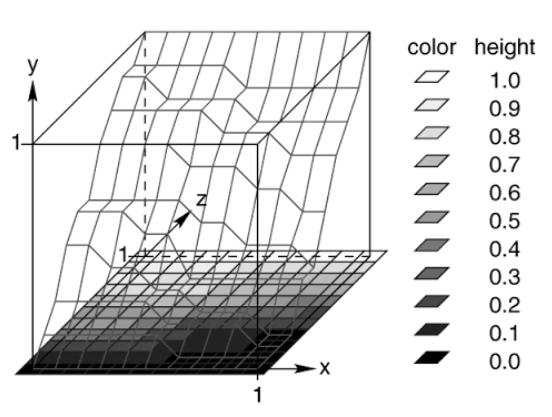
\includegraphics[width=0.6\linewidth]{Height field.png}\hspace*{\fill}
\caption{Výškové pole}
\label{fig:heightfield}
\end{figure}



Výšková pole jsou struktura používaná v mnoha reálných aplikacích. Například v rámci modelování může být použito k bump mappingu, iluzi nerovnosti povrchu bez změny jeho geometrie, kde se výškové pole používá k vypočítání stínů v materiálu. Také se používá při displacement mappingu, kdy se skutečně mění geometrická poloha objektu, a při modelování terénů, jako v této práci.

K renderování výškových polí se stále často používá převedení výškového pole do alternativní reprezentace. Nejčastěji se jedná o převedení do polygonové sítě, ale existují i méně běžné varianty, jako převedení do množiny bodů nebo objemové reprezentace, vše pro maximální využití konkrétního hardware rendereru.


\begin{figure}[h]
\hfill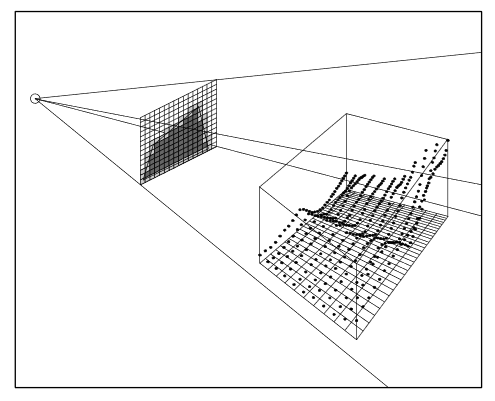
\includegraphics[width=0.6\linewidth]{rtfrustum.png}\hspace*{\fill}
\caption{Pohledový jehlan na výškové pole}
\label{fig:raytracing}
\end{figure}



Přímé renderování pomocí ray tracingu (viz obrázek \ref{fig:raytracing}) může mít své výhody. Strukturu je možné uložit ve stručnější reprezentaci než jsou derivované geometrické nebo objemové verze. Ze své podstaty ignoruje neviditelné oblasti a získává důležité informace o struktuře, které mohou být použity ke zrychlení procesu rozhodování, zda a kdy se objevil průsečík.


\begin{figure}[h]
\hfill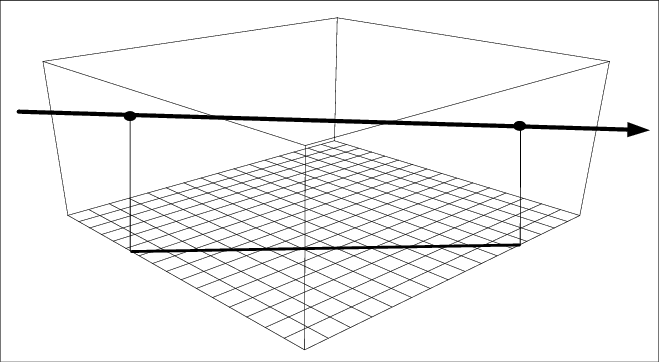
\includegraphics[width=0.6\linewidth]{Projection-of-the-ray-onto-the-height-field-base-plane.png}\hspace*{\fill}
\caption{Průmět paprsku na mřížku}
\label{fig:prumet}
\end{figure}


Aby vůbec existoval průsečík paprsku a výškového pole, musí existovat průsečík paprsku a ohraničujícího kvádru výškového pole (viz obrázek \ref{fig:prumet}). Pokud existuje, algoritmus pokračuje a promítne paprsek na základní rovinu výškového pole. Paprsek se poté dá procházet v mřížce například pomocí Digitálního rozdílového analyzátoru (DDA), algoritmu středního bodu, nebo právě metodou úseků, kterou používám dále.


\begin{figure}[h]
\hfill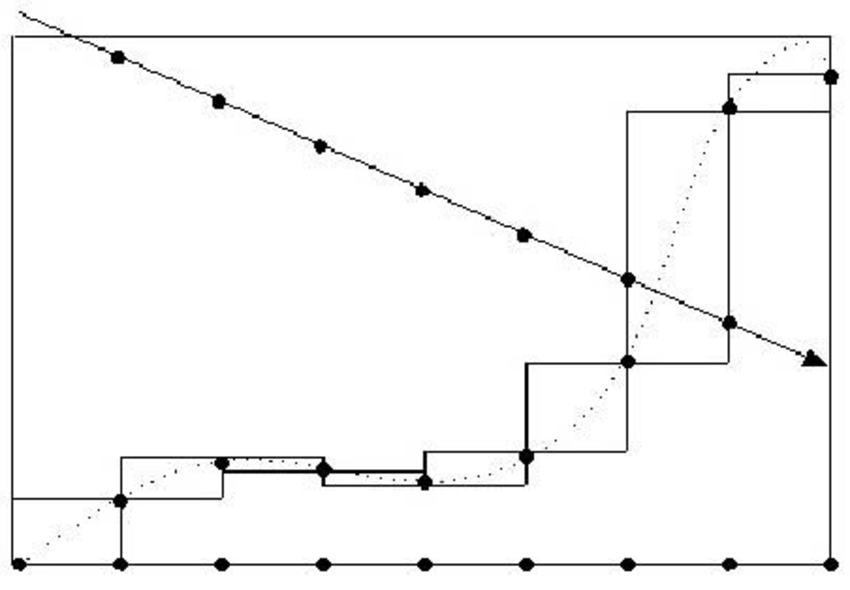
\includegraphics[width=0.6\linewidth]{Intersecting-the-ray-with-the-bounding-heights-of-neigh-boring-cells.png}\hspace*{\fill}
\caption{Průsečík paprsku s ohraničujícími kvádry buňky}
\label{fig:z}
\end{figure}


Jakmile známe buňky na trase průmětu paprsku v mřížce, je možné aplikovat různé strategie pro nalezení průsečíku. Může být testována výška paprsku proti vzorkům buněk (viz obrázek \ref{fig:z}), nebo může být zkonstruována polygonální reprezentace povrchu. Pole samotné pak vykreslujeme například za použití texturové mapy nebo lokálního modelu osvětlení, který je použitý i v této práci.

Procházíme tedy průmět paprsku v souřadném systému výškového pole, kde výška i šířka buňky je 1. Dráha paprsku tak je \[y = \alpha x + \beta; \; \alpha, \beta \in R\] a použijeme princip digitální přímky. Jediný rozdíl je, že paprsek je, na rozdíl od přímky, nekonečný jen v jednom směru. Uvažujeme osmispojité sousedství, jako v principu digitální přímky, ale sekvence, do nichž paprsek nevstupuje rohem, se musí prodloužit o délku jedné buňky v rovině úseku, abychom zjistili, zda zde přímka neprotíná výškové pole (dle obrázku \ref{fig:connected}).


\begin{figure}[h]
\hfill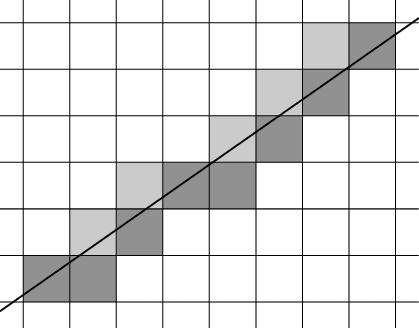
\includegraphics[width=0.35\linewidth]{The-minimal-8-connected-definition-of-the-line.png}\hspace*{\fill}
\caption{4- a 8-spojitá digitální přímka}
\label{fig:connected}
\end{figure}

\begin{figure}[h]
\hfill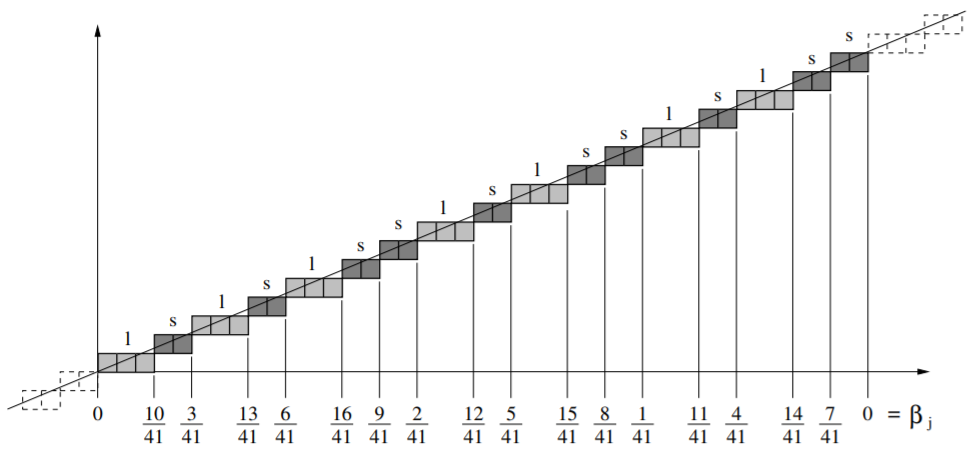
\includegraphics[width=0.8\linewidth]{The-structure-of-runs-within-the-digital-line-y-17-41-x.png}\hspace*{\fill}
\caption{Příklad nalezení úseků přímky se směrnicí 17/41}
\label{fig:example}
\end{figure}

Digitalizovaný paprsek je složen z úseků, tedy množin souvislých buněk se stejnou souřadnicí y. Tyto úseky tedy sousedí právě jedním rohem. Abychom popsali strukturu úseků v digitálním paprsku, zaměříme se na přímku s racionální směrnicí, která umožňuje opakování posloupnosti délek úseků. Tato směrnice je definována na segmentu přímky, který začíná a končí přímo v rozích mřížky (viz příklad na obrázku \ref{fig:example} se směrnicí 17/41, \(\beta _j\) je vysvětleno dále). Racionální směrnice \(\alpha\) je tedy
\[\alpha = \delta y / \delta x\]
kde \(\delta y\) je počet úseků ve výše definovaném segmentu a \(\delta x\) počet buněk v něm.

Zaměřujeme se tedy zatím na přímku s nulovým průsečíkem, tedy dráha paprsku bude
\[y = \alpha x\]
Dále volíme příklad, kdy \(\alpha\) je mezi 0 a 1 a paprsek vchází do mřížky zleva. Ostatní případy řešíme například transformacemi kartézského systému souřadnic. Další postup je naznačen za pomoci pseudokódu.

Úseky tedy určujeme pomocí počátečního bodu x, y, dále značených jako \verb|currentX| a \verb|currentY| a současné délky úseku, značené jako  \verb|currentRunLength|. Následující x a y získáme tedy jako:

\begin{verbatim}
currentX = currentX + currentRunLength
currentY = currentY + 1
\end{verbatim}

Úseky se v přímce vyskytují maximálně ve dvou délkách, které jsou po sobě jdoucí celá čísla. Z informací zmíněných výše lze odvodit, že délka krátkých úseků je 
\begin{verbatim} runLengthShort = floor(1 / alpha) \end{verbatim}
a délka dlouhých
\begin{verbatim} runLengthLong = ceil(1 / alpha) \end{verbatim}

Klíčové je tedy získat délku následujícího úseku. Tu můžeme určit pomocí intercepční posloupnosti. Intercepční posloupnost je posloupnost hodnot \(\beta _j\), která říká, jak vysoko od spodní hrany buňky vstupuje paprsek do j-tého úseku. Tedy \(0 \leq \beta _{j} < 1\). V úseku je to právě hodnota \(\beta _j\), která rozhoduje, zda bude úsek dlouhý nebo krátký. Pro začátek úseku dokonce platí \(0 \leq \beta _{j} < \alpha\). Tuto hodnotu značíme dále v pseudokódu jako \verb|currentIntercept|. Následující hodnotu \(\beta _{j+1}\) získáme z alfy a současné délky úseku jako
\begin{verbatim}
currentIntercept = currentIntercept + alpha * currentRunLength - 1
\end{verbatim}


\begin{figure}[h]
\hfill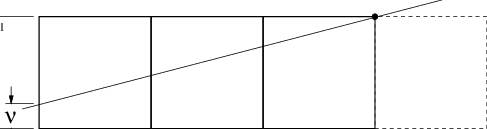
\includegraphics[width=0.6\linewidth]{The-geometry-of-the-intercept-of-a-run-and-the-line.png}\hspace*{\fill}
\caption{Geometrie interceptu úseku a přímky}
\label{fig:geom}
\end{figure}


Následnou délku úseku pak zjistíme podle toho, zda je vypočtená \(\beta _{j+1}\) vyšší nebo nižší než hodnota v, což je hodnota zobrazená na obrázku \ref{fig:geom}. Ta značí, jaký je \(\beta _{j}\), když přímka protíná pravý horní roh dlouhého úseku. Jedná se tedy o limit, kde pokud je \(\beta _{j+1}\) pod ním, je následující úsek dlouhý, pokud na ním, je krátký. Vypočteme ji jako
 \begin{verbatim} v = 1 - alpha * runLenghtShort \end{verbatim}
 a následující délku úseku určíme jako
 \begin{verbatim}
currentRunLength = (currentIntercept < v) ? runLengthLong : runLengthShort
 \end{verbatim}
 
 
 Dále zbývá vypočítat pouze vstupní posun promítnutého paprsku. Zde počítáme s bodem, kde paprsek vstupuje do mřížky, dále značeným jako \verb|from|, z něj určíme oříznutím na celé číslo i počáteční hodnoty \verb|currentX| a \verb|currentY|. Nejprve vypočteme \(\beta\), obdobně jako je definováno \(\beta _{j}\)
 \begin{verbatim}
 beta = from.y - floor(from.y)
 \end{verbatim}
 kde odečteme od skutečné souřadnice polohu dolní hrany buňky v mřížce. Zde tedy platí, že je hodnota kdekoli mezi 0 a 1. Pokud je tato hodnota nad maximální hodnotou \(\beta _{j}\) (tedy \(\alpha\)), znamená to, že je první úsek zkrácen. Zkrácení z dlouhého na krátký zvlášť nezohledňujeme, tedy první úsek je zkrácený, pokud
 \begin{verbatim}
 beta >= alpha + v
 \end{verbatim}
 Délku tohoto úseku, značenou \verb|lengthOfTruncated|, určíme jako
 \begin{verbatim}lengthOfTruncated = ceil((1 - beta) / alpha)\end{verbatim}
 V tomto úseku také hledáme průsečík a následně počítáme délku a hodnotu následující posloupnosti. Tento postup je zobrazen v pseudokódu níže.
 
\begin{verbatim}
 if (beta >= alpha + v)
    lengthOfTruncated = ceil((1 - beta) / alpha)
    // --> search for intersection in run 0 - length of truncated
    if (findInRun(0, lengthOfTruncated, currentY, ...))
        return true;
    currentX += lengthOfTruncated;
    currentY += 1;
    currentIntercept = (beta - v) - (alpha * floor((beta - v) / alpha));
    currentRunLength = (currentIntercept < v)
      ? runLengthLong
      : runLengthShort;
\end{verbatim}
Po tomto výpočtu algoritmus pokračuje v cyklu, dokud nenarazí na průsečík nebo nedojde do konce mřížky. Tělo uvnitř cyklu je zobrazeno v následujícím pseudokódu, \verb|widthOfGrid| je počet buněk na šířku mřížky.

\begin{verbatim}
    if (findInRun(
          max(0, currentX - 1),
          min(currentX + currentRunLength, widthOfGrid),
          currentY,
          ...)
    ) {
      return true;
    }
    currentX += currentRunLength;
    currentY += 1;
    currentInterceptBeta += alpha * currentRunLength - 1;
    currentRunLength = (currentInterceptBeta < v)
      ? runLengthLong
      : runLengthShort;
\end{verbatim}

Pokud algoritmus nenalezl průsečík v cyklu, průsečík neexistuje.

 
 Nakonec zbývá jen rekonstrukce povrchu, pro kterou algoritmus používá aproximaci pomocí dvou trojúhelníků se vzorky výšky mřížky jako vrcholy trojúhelníků.


Algoritmus je k nahlédnutí zde: \url{https://github.com/stetizu1/DPG-semestral-project}

V rámci této práce jsem naimplementovala vlastní ray tracer. Práce používá knihovny Freeglut, OpenGL a Corona pro čtení obrázků.

%%%% -------------------------------------------------------- 
\section{\label{SEC:Pitfalls}Potíže při implementaci}

Mým největším problémem bylo, že algoritmus, který jsem chtěla zpracovávat, nebyl v paperu příliš dobře popsán. Často jsem tápala a nevěděla, co tím autor myslí a paper jsem si musela číst hned několikrát. Stále si nejsem jistá, zda jsem správně porozuměla všem jeho detailům -- pro někoho nezkušeného s čtením profesionálních článků o grafice to není úplně ideální začátek.

Při praktické implementaci mi činil potíže fakt, že autor vysvětluje výpočet pouze pro jednu šestnáctinu možných případů, kdy paprsek zrovna přichází do výškového pole do první buňky zleva, se směrnicí mezi 0 a 1. Převod ostatních případů pak vysvětluje jednou větou, která pouze říká, že vzhledem k symetrii kartézského prostoru lze tuto přímku transformovat na všechny případy, nikoli však jak a už vůbec ne jak efektivně. Díky tomu nevím, zda je moje řešení dostatečně efektivní. Implementovala jsem algoritmus pro všechny paprsky, které do výškového pole přichází z nulových souřadnic (x nebo z paprsku na vstupu je rovno 0). Příklady jsou vybrány tak, aby s tím počítaly. Pro případné rozšířeni stačí přidat transformaci počítající od konce na začátek.

Dalším výrazným problémem bylo, že algoritmus popsaný v paperu počítal jen s racionálními čísly, což při převodu na float způsobilo výrazné chyby v zaokrouhlení. Vytvořila jsem si tak typ pro racionální čísla, který při zvolení vhodné přesnosti vytváří znatelně kvalitnější výsledky než float.

Na druhou stranu data výškových polí byla velmi jednoduchá získat, k debugování šlo použít i vlastnoručně vyrobené obrázky.

Celá práce mi i se studiem článku, psaním ray traceru, testováním a psaním dokumentace zabrala kolem 160 hodin.

%%%% -------------------------------------------------------- 
\section{\label{SEC:Results}Naměřené výsledky}
%\section{\label{SEC:Results}Results}

Do tohoto dokumentu přikládám výběr 3 obrázků, na nichž jsem algoritmus testovala, a které jsem vybrala jako vzorové. Jejich renderování je možné spustit pomocí přiložených bat souborů. Konkrétně jde o náhodný vzorek z Čech (obrázek \ref{fig:sample}), Grand Canyon (obrázek \ref{fig:gc}) a část Šumavy (obrázek \ref{fig:sum}). Uvedla jsem zde i jejich výšková pole, viz respektive obrázky \ref{fig:sampleHm}, \ref{fig:gcHm} a \ref{fig:sumHm}.

Velikost výškových polí těchto obrázků je 49x49 pro první vzorek, 500x500 pro vzorek Šumavy a 434x434 pro Grand Canyon. Scény s těmito poli jsou scéna 0, kde je vzorek z Čech, scéna 1, kde je Grand Canyon a scéna 2, kde se nachází Šumava.


\begin{figure}[h]
\hfill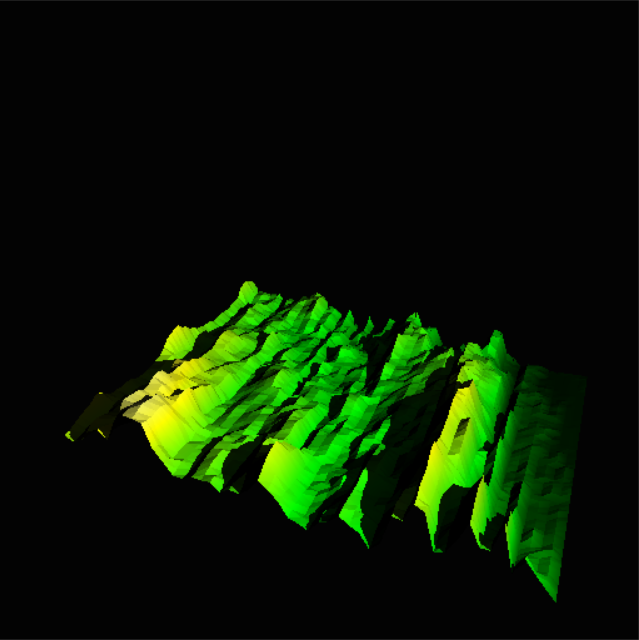
\includegraphics[width=0.6\linewidth]{field.png}\hspace*{\fill}
\caption{Vzorek z Čech}
\label{fig:sample}
\end{figure}



\begin{figure}[h]
\hfill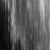
\includegraphics[width=0.3\linewidth]{vzorek.png}\hspace*{\fill}
\caption{Vzorek z Čech - výškové pole}
\label{fig:sampleHm}
\end{figure}


\begin{figure}[h]
\hfill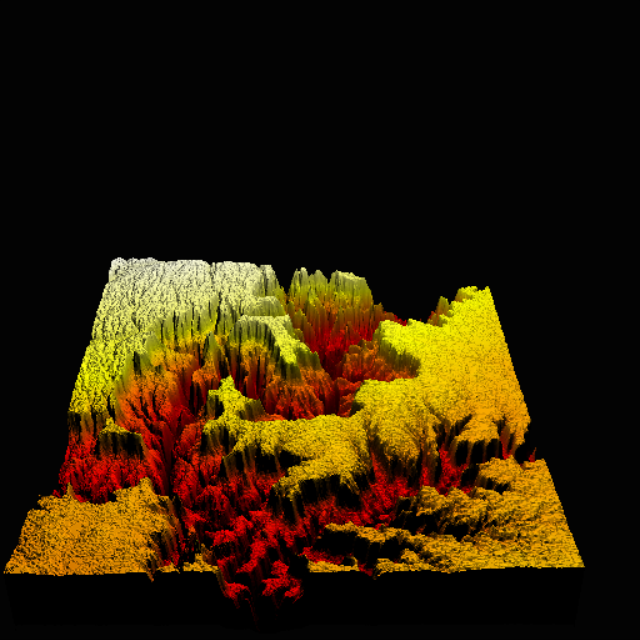
\includegraphics[width=0.6\linewidth]{grand_canyon.png}\hspace*{\fill}
\caption{Grand Canyon}
\label{fig:gc}
\end{figure}

\begin{figure}[h]
\hfill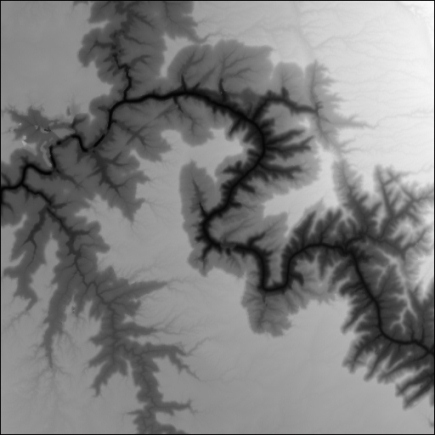
\includegraphics[width=0.5\linewidth]{grand_canyon.jpg}\hspace*{\fill}
\caption{Grand Canyon - Výšková pole}
\label{fig:gcHm}
\end{figure}

\begin{figure}[h]
\hfill\includegraphics[width=0.6\linewidth]{sumava.png}\hspace*{\fill}
\caption{Šumava}
\label{fig:sum}
\end{figure}


\begin{figure}[h]
\hfill
\includegraphics[width=0.4\linewidth]{Sumava.png}\hspace*{\fill}
\caption{Šumava - výškové pole}
\label{fig:sumHm}
\end{figure}

Po dokončení práce jsem postoupila k měřením. Jako první jsem měřila rychlost postavení datové struktury, viz tabulka \ref{tab:measurementT1}. Měřila jsem rychlost postavení struktur velikostí 100x100, 200x200, 300x300, 400x400 a 500x500 a to pro počet postavení 1, 10, 100 a 1000 struktur. Každé měření rychlosti bylo provedeno minimálně pětkrát a byl vypočten průměr.

\begin{table}
\begin{tabular}{| l || r | r | r | r |}
\hline\bfseries Počet postavení DS & \bfseries 1 & \bfseries 10 & \bfseries 100 & \bfseries 1000 \\
\bfseries Velikost výškového pole & [ms] & [ms] & [ms] & [ms] \\ \hline
\bfseries 500x500 & 55 & 523 & 5 109 & 45 584 \\ \hline
\bfseries 400x400 & 36 & 337 & 3 314 & 29 105 \\ \hline
\bfseries 300x300 & 19 & 190 & 1 825 & 16 074 \\ \hline
\bfseries 200x200 & 9 & 85 & 816 & 7 228 \\ \hline
\bfseries 100x100 & 2 & 20 & 198 & 1 862 \\ \hline
\end{tabular}
\caption{Měření rychlosti postavení datové struktury}
\label{tab:measurementT1}
\end{table}

Dále jsem na měření používala ukázkové scény, které jsou uvedeny výše. S nimi jsem jako první měřila dobu postavení DS a dobu výpočtu výsledného obrazu (výpočet ray tracingu), tedy čas po postavení datové struktury, do té doby než je vyplněn celý obraz barvou, shrnuto v tabulce \ref{tab:measurementT2}.

\begin{table}
\begin{tabular}{| l || r | r |}
\hline
\bfseries Čas & \bfseries Postavení DS & \bfseries Výpočet \\
\bfseries Scéna & [ms] & [ms] \\ \hline
\bfseries 0 & 1 & 1 142 \\ \hline
\bfseries 1 & 29 & 5 183 \\ \hline
\bfseries 2 & 40 & 9 342 \\ \hline
\end{tabular}
\caption{Měření rychlosti na ukázkových scénách}
\label{tab:measurementT2}
\end{table}


Dále jsem testovala počet dotazů na průsečík mezi výškovým polem a paprskem ve třech přiložených scénách, zaznamenáno v tabulce \ref{tab:measurementN1}. V tabulce uvádím počet dotazů dle toho, na co byly určeny. První sloupeček určuje počet primárních paprsků, druhý počet dotazů na průsečík paprsku a ohraničujícího kvádru (primární + stínové), třetí počet dotazů na průsečík mezi paprskem a buňkou a poslední mezi paprskem a trojúhelníkem.

\begin{table}
\begin{tabular}{| l || r | r | r | r |}
\hline
\bfseries Počet dotazů &  \bfseries Primární paprsky &  \bfseries Ohraničující kvádr &  \bfseries Buňka &  \bfseries Trojúhelník \\
\bfseries Scéna &  &  &  & \\ \hline
\bfseries 0 & 262 144 & 317 129 & 6 820 710 & 8 395 121 \\ \hline
\bfseries 1 & 262 144 & 369 971 & 41 770 313 & 59 552 379 \\ \hline
\bfseries 2 & 262 144 & 317 643 & 53 175 433 & 43 853 800 \\ \hline
\end{tabular}
\caption{Měření počtu dotazů}
\label{tab:measurementN1}
\end{table}

K této tabulce dodávám i přepočet poměru ostatních dotazů na jeden primární paprsek, do tabulky \ref{tab:measurementN2}.

\begin{table}
\begin{tabular}{| l || r | r | r |}
\hline
\bfseries Průměrný počet dotazů na primární paprsek & \bfseries Ohraničující kvádr &  \bfseries Buňka &  \bfseries Trojúhelník \\
\bfseries Scéna & & & \\ \hline
\bfseries 0 & 1,21 & 26,02 & 32,02 \\ \hline
\bfseries 1 & 1,41 & 159,34 & 227,17 \\ \hline
\bfseries 2 & 1,21 & 202,85 & 167,29 \\ \hline
\end{tabular}
\caption{Poměr dotazů na jeden primární paprsek}
\label{tab:measurementN2}
\end{table}

V návaznosti jsem zjistila, kolik dotazů na průsečík je vyhodnoceno jako pravda a kolik se vyhodnotí jako nepravda a určila poměr mezi nimi a zaznamenala jej do tabulky \ref{tab:measurementN3}. Zde E značí počet nalezených průsečíků (existuje) a N počet dotazů, které nenašly průsečík (neexistuje). Poměr E/N značí kolik hledání bylo vyhodnoceno neúspěšně na jedno úspěšné. U primárních paprsků se jedná o celkový počet těch, které našly průsečík s výškovým polem, proti těm, které takový průsečík nemají.

\begin{table}
\begin{tabular}{| l || r | r | r | r |}
\hline\bfseries Počet dotazů / scéna &  \bfseries Primární paprsky &  \bfseries Ohraničující kvádr &  \bfseries Buňka &  \bfseries Trojúhelník \\ \hline

\bfseries 0 - E  & 54 985 & 157 140 & 109 672 & 109 672 \\
\bfseries 0 - N  & 207 159 & 159 989 & 6 711 038 & 8 285 449 \\
\bfseries 0 - E/N  & 3,77 & 1,02 & 61,19 & 75,55 \\ \hline

\bfseries 1 - E  & 107 827 & 233 585 & 128 417 & 128 417 \\
\bfseries 1 - N  & 154 317 & 136 386 & 41 641 896 & 59 423 962 \\
\bfseries 1 - E/N  & 1,43 & 0,58 & 324,27 & 462,74 \\ \hline

\bfseries 2 - E  & 55 499 & 150 374 & 110 997 & 110 997 \\
\bfseries 2 - N  & 206 645 & 167 269 & 53 064 436 & 43 742 803 \\
\bfseries 2 - E/N  & 3,72 & 1,11 & 478,07 & 394,09\\ \hline
\end{tabular}
\caption{Měření počtu dotazů}
\label{tab:measurementN3}
\end{table}

Naměřená data tak odpovídají předpokladům, co se týče průměrné složitosti na traverzaci paprsku. Konkrétní výsledky pak závisí na nastavení pohledu na výškové pole.

Implementace běží na jednom jádru.

Data byla měřena na této sestavě:
\begin{itemize}
    \item CPU: Intel(R) Core(TM) i9-10900K
    \begin{itemize}
        \item 3.7 GHz
        \item 10 cores
        \item 64K L1 cache per core, 256K L2 cache per core, 20MB L3 cache
    \end{itemize}
    \item RAM 64 GB
\end{itemize}

Program byl vyvíjen a testován na operačním systému Windows 10, při vývoji jsem používala kompilátor MSVC (uvnitř CLionu).


%%%% -------------------------------------------------------- 
\section{\label{SEC:Conclusion}Závěr}

Implementování této práce mě mnoho naučilo. Ačkoli jsem nepoužívala nejmodernější algoritmus (paper je z roku 2004), měl jistě zajímavou myšlenku. Ráda bych si někdy zkusila implementovat i nějaký jiný přístup, který se dnes na tento problém používá.

Samotná implementace mě bavila, základ ray traceru, který jsem napsala, by dle mého názoru šel použít i v rámci jiných algoritmů hledání průsečíků. V práci je rozhodně i prostor k vylepšení, snažila jsem se tak i o co nejlepší dokumentaci metod, abych se k ní mohla kdykoli vrátit.

Kdybych na práci měla více času, jistě bych jí ještě nějaký věnovala, ale i v tomto stavu jsem nad ní strávila dle mého názoru dostatek času (zhruba 160 hodin celkově).


\end{document}
